%% Sections 1-2: Introduction; Data and methods (with Figure 1 and Table 1)

\section{Introduction}\label{sec:intro}

The Silk Nebula is a faint \Oiii~$\lambda$5007 filament in Gemini (Figure~\ref{fig:overview}). Its ridge follows a $16.9^\circ$ arc from $(\ell,b)\approx(208^\circ,+17.5^\circ)$ to $(191^\circ,+21.8^\circ)$ with a full width at half maximum (FWHM) of $0.28^\circ$; a second strand (W) branches west from the main strand (E, the spine) near declination (Dec) $+15^\circ$.

Several groups found the filament independently. The Super Wide-Field \Oiii\ Narrowband Survey (SWONS) team detected it in late 2023 and named it the Silk Nebula \citep{QHYCCD2024}; a team member posted the first public image on 2024 January~14.\footnote{AstroBin image \url{https://www.astrobin.com/zh47r9/}.} The Northern Sky Narrowband Survey (NSNS) recorded the full arc and gave the first journal description \citep{Ziegenbalg2025}, and \citet{Fesen2026} imaged it as part of the eastern and northern limbs of the Monogem Ring.

\citeauthor{Wu2026} (\citeyear{Wu2026}; hereafter W26) used 2,684 spectra at $R\sim7500$ from one plate of the Medium-Resolution Spectroscopic Survey of Nebulae (MRS-N; \citealt{Wu2022}) of the Large Sky Area Multi-Object Fiber Spectroscopic Telescope (LAMOST; \citealt{Cui2012}), observed on 2024 February~1, and analyzed three regions on the filament (P1--P3) and a nebula-free background (P4). The blue arm (4950--5350\,\AA) covers \Oiii~$\lambda\lambda$4959, 5007 but not \Hb; the red arm (6300--6800\,\AA) covers \Ha, \Nii\ and \Sii. W26 concludes that the filament is possibly associated with a supernova remnant (SNR) at a fiducial distance of $\sim$160\,pc, where it is $\sim$28\,pc long, with energy $(2.0\pm0.7)\times10^{51}$\,erg and age $(6.8\pm1.8)\times10^{4}$\,yr, and notes that a diffuse-ionized-gas (DIG) or ionized-bubble origin cannot be ruled out.

\begin{figure*}
\centering
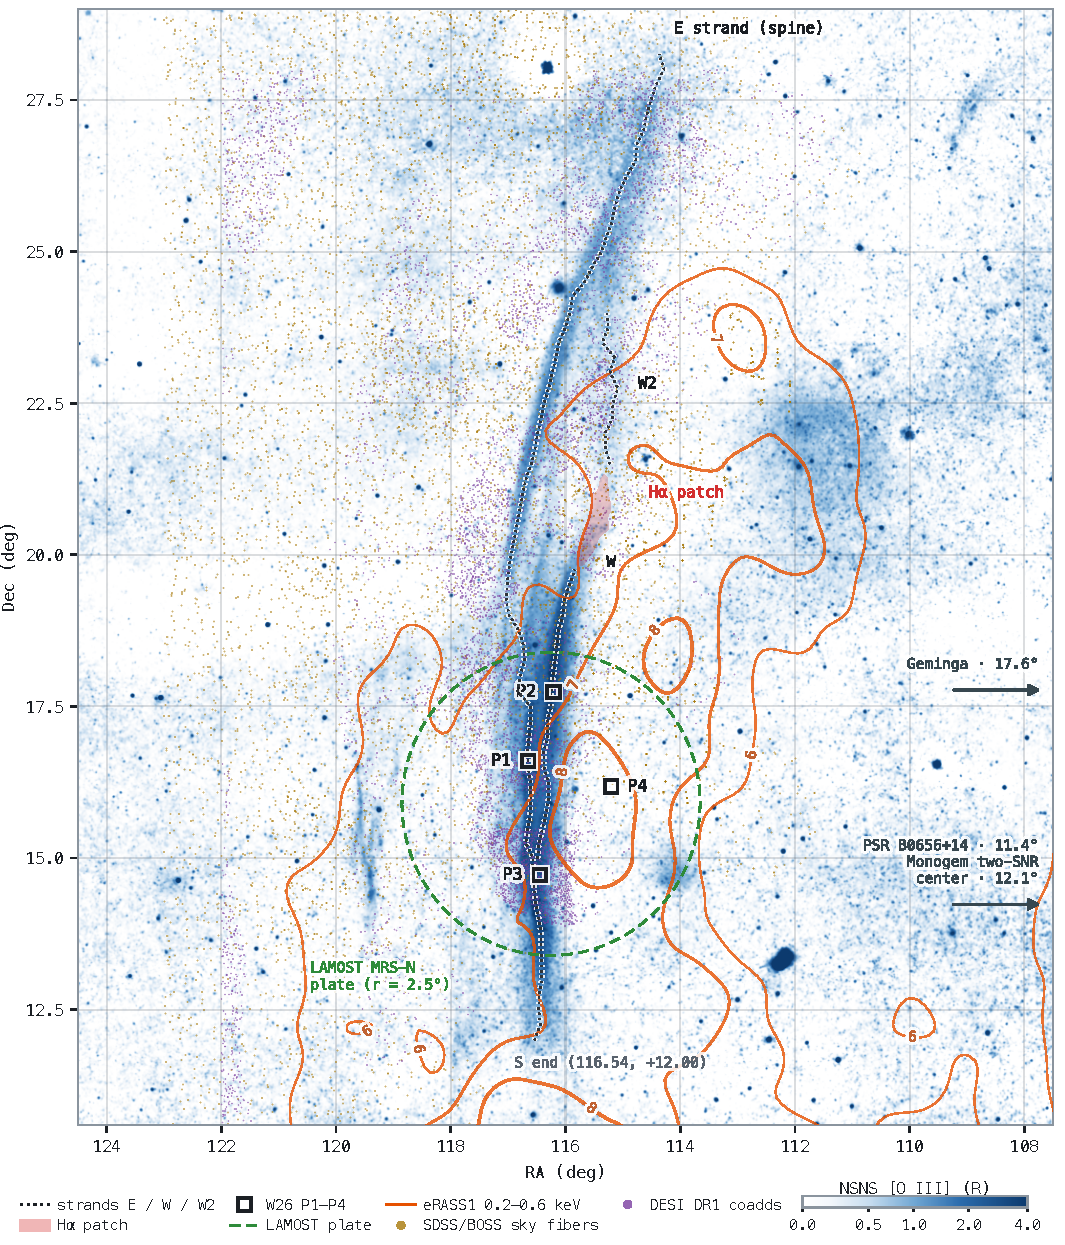
\includegraphics[width=0.9\textwidth]{figures/w3_figs_f1_overview.pdf}
\caption{The Silk Nebula on the NSNS DR0.2 \Oiii~$\lambda$5007 map \citep{Ziegenbalg2025}, in rayleighs (R; arcsinh scale). Dotted lines: the E (spine), W and W2 strands. Shaded polygon: half-maximum outline of the \Ha\ patch in NSNS \Ha\ imaging. Squares: regions P1--P4 of W26 \citep{Wu2026}; dashed circle: the LAMOST MRS-N plate ($2.5^\circ$ radius). Contours: 0.2--0.6\,keV surface brightness of the first SRG/eROSITA all-sky survey (eRASS1; \citealt{Merloni2024}) at 6, 7 and 8\,counts\,s$^{-1}$\,deg$^{-2}$, after masking point sources and smoothing. Dots: the SDSS/BOSS sky fibers \citep{Abdurrouf2022,SDSS2026} and DESI DR1 coadds \citep{DESI2026} analyzed here. Arrows point toward Geminga, and toward PSR B0656+14 and the two-remnant Monogem center of \citet{Knies2024}; labels give the mean angular distance of the spine from Geminga, and of its southern part (Dec $<17.6^\circ$) from the other two.}
\label{fig:overview}
\end{figure*}

Independent data support two W26 results: the \Oiii\ filament is real line emission, absent from P4, and the red-arm lines trace foreground and background warm ionized medium (WIM), the DIG of W26 Sect.~4.2.

The SNR interpretation, however, rests on red-line diagnostics and the \Oiii\ morphology; the size, energy and age derived for it rest on line velocities and a kinematic distance, and W26 also quotes a surface brightness. We test each of these against W26's published values and independent data, chiefly archival spectra from the Dark Energy Spectroscopic Instrument (DESI) and the Sloan Digital Sky Survey (SDSS), which also cover \Hb, \Oii\ and \ion{He}{2}, and add new constraints on the filament's excitation and location.

Section~\ref{sec:data} describes the data and methods. Sections~\ref{sec:assess} and \ref{sec:new} assess the W26 claims (Table~\ref{tab:claims}) and present new constraints; Section~\ref{sec:future} proposes decisive observations, and Section~\ref{sec:conclusions} concludes.

\begin{deluxetable*}{llc}
\tablecaption{W26 claims assessed in this work\label{tab:claims}}
\tablehead{\colhead{Claim (W26 location)} & \colhead{Our finding} & \colhead{Section}}
\startdata
\parbox[t]{0.36\textwidth}{\raggedright \Oiii\ \vhel\ $+23.8$ to $+26.8$\,\kms, 5--15\,\kms\ above the red lines; two-layer shell (Table~4; Sects.~3.2.3, 4.2)\strut} & \parbox[t]{0.48\textwidth}{\raggedright The blue-arm scale is air and topocentric, so Table~4 \Oiii\ is $10.1\pm1.0$\,\kms\ too high; \Oiii\ lies at $+13.3\pm1.0$\,\kms, $+1.1\pm1.3$\,\kms\ from \Nii\strut} & \S\ref{sec:oiii} \\
\parbox[t]{0.36\textwidth}{\raggedright \Ha\ \vhel\ $+16.3$ to $+19.7$\,\kms, used for velocities, the velocity map and distances (Table~4; Fig.~5)\strut} & \parbox[t]{0.48\textwidth}{\raggedright \Ha\ exceeds \Nii\ by $5.5\pm1.1$\,\kms\ and WHAM by $4.8\pm0.7$\,\kms; a geocoronal over-subtraction model reproduces one-half to three-quarters\strut} & \S\ref{sec:halpha} \\
\parbox[t]{0.36\textwidth}{\raggedright Fiducial distance $\sim$160\,pc from \Oiii\ kinematic distances ``in units of 100pc'' (Table~4; Sect.~3.3)\strut} & \parbox[t]{0.48\textwidth}{\raggedright Table~4 values are reproduced only as kpc ($\sim$1.6\,kpc); rotation gives $\le3.1$\,\kms\ within 300\,pc, below peculiar motions\strut} & \S\ref{sec:distance} \\
\parbox[t]{0.36\textwidth}{\raggedright \Oiii\ 23.60--23.87\,mag\,arcsec$^{-2}$, i.e., $\sim$10--13\,R (Table~3; Sect.~4.1)\strut} & \parbox[t]{0.48\textwidth}{\raggedright Exceeds DESI, SDSS and NSNS values (1.4--2.5\,R) by factors of 4.6--8.6; no identified multiplicative systematic accounts for this\strut} & \S\ref{sec:brightness} \\
\parbox[t]{0.36\textwidth}{\raggedright Shock excitation from \Sii/\Ha\ $>0.4$, \Nii/\Ha\ and diagnostic diagrams (Abstract; Sect.~4.1; Fig.~8)\strut} & \parbox[t]{0.48\textwidth}{\raggedright Ratios in nebula-free P4 equal those on the filament within $1\sigma$ and match faint high-latitude WIM\strut} & \S\ref{sec:shock} \\
\parbox[t]{0.36\textwidth}{\raggedright $n_e$, $T_e$, $V_t$, O/H, \Oiii\ widths, energetics and radio non-detection (Sects.~3.2--4.1; Tables~2, 4)\strut} & \parbox[t]{0.48\textwidth}{\raggedright Table~2 ratios imply $n_e=225$--631\,cm$^{-3}$; $T_e$ ($\sigma_T=7300$--10700\,K), $V_t$ and O/H are consistent with P4; widths not recoverable at S/N~6; energetics inputs unsupported; NVSS/TGSS resolve the filament out\strut} & \S\ref{sec:snrdiag}
\enddata
\tablecomments{Table, figure and section numbers in the first two columns refer to W26. Velocities are heliocentric. P4 is the nebula-free background region of W26. WHAM, Wisconsin H$\alpha$ Mapper; WIM, warm ionized medium; $n_e$, electron density; $T_e$, electron temperature ($\sigma_T$, its $1\sigma$ uncertainty); $V_t$, turbulent velocity.}
\end{deluxetable*}

\section{Data and methods}\label{sec:data}

\subsection{W26 material}

We use W26 arXiv version~1, whose tables match the journal version. We extracted the W26 Fig.~3 spectra and the \Ha\ \vlsr\ map of W26 Fig.~5 from the PDF vector data (spectral axes calibrated to 0.002\,\AA\ rms), and digitized the \Oiii\ \vlsr\ histogram of the same figure. The per-fiber MRS-N nebular spectra are not public \citep{Zhang2025}, so our corrections to W26 values apply in aggregate.

\subsection{Archival spectra}

\emph{DESI DR1.} The DESI pipeline \citep{Guy2023} subtracts a sky model built from the sky fibers of each petal and exposure, so the filament leaves positive residuals on the ridge and negative ones elsewhere on its petals. In $\pm40$\,\AA\ line windows of 7,620 DR1 coadds \citep{DESI2026} near the filament and in control fields $>5^\circ$ away, we subtracted each target's pipeline model and regressed each line residual on that predicted for Gaussian ridges along the traced strands, minus the tile--petal mean (a proxy for the sky-fiber mean). This isolates emission correlated with the filament, canceling smooth WIM and sky, and gives the \Oiii\ intensity and line ratios relative to \Oiii. HEALPix block-bootstrap uncertainties are inflated to match line-free null windows, and the [\ion{O}{1}]~$\lambda$5577 sky line gauges template-correlated systematics. Surface brightness uses the per-exposure guide-camera point-source fiber acceptance (median 0.566 at 5008\,\AA; $\pm8\%$ systematic, or $\approx$20\% for two survey-validation tiles that lack guide-camera data; Appendix~\ref{sec:appendix-desi}).

\emph{SDSS sky fibers.} We used 9,092 sky-fiber spectra from SDSS-I/II, BOSS and eBOSS (DR17; \citealt{Abdurrouf2022}) and SDSS-V (DR19; \citealt{SDSS2026}), in 302 plate--night--spectrograph groups (250 dark). Because \Oiii~$\lambda$5007 and \Hb\ have no significant airglow, the total sky (pipeline residual plus sky model) measures them absolutely. ON$-$OFF differences within each group (ON within $0.15^\circ$ of a strand, OFF at $0.45^\circ$--$2.0^\circ$) cancel plate-level systematics, [\ion{O}{1}]~$\lambda$5577 sets the velocity zero points, and shifted-trace placebos calibrate residual systematics. Matching to SDSS imaging sky levels \citep{Almeida2023} gives diffuse-light correction factors of $0.84\pm0.08$ for 3\arcsec\ and $0.60\pm0.06$ for 2\arcsec\ fibers.

\subsection{Imaging and ancillary data}

We traced the ridge (66 points at $0.25^\circ$ declination steps; median uncertainty $0.022^\circ$) on W26 Figs.~1 and 4 and the NSNS DR0.2 maps \citep{Ziegenbalg2025}, registered to Tycho-2 stars \citep{Hog2000}; the NSNS calibration is adopted as published. Ancillary data are GALEX far- and near-ultraviolet (FUV, NUV) images \citep{Martin2005,Morrissey2007}, in continuum units (CU; photons\,cm$^{-2}$\,s$^{-1}$\,sr$^{-1}$\,\AA$^{-1}$); \Ha\ from the Southern H-Alpha Sky Survey Atlas (SHASSA; \citealt{Gaustad2001}) and the Wisconsin \Ha\ Mapper (WHAM; \citealt{Haffner2003}); the Galactic Arecibo L-band Feed Array \ion{H}{1} survey (GALFA-\ion{H}{1}) DR2 \citep{Peek2018}; the IRIS reprocessing of the IRAS 100\,$\mu$m maps \citep{MivilleDeschenes2005}; SRG/eROSITA eRASS1 0.2--0.6\,keV maps \citep{Merloni2024}; and the FIMS/SPEAR \ion{C}{4} map of \citet{Kim2007}, digitized from the published figure. Counterpart tests use cross-filament profiles and template regressions on the \Oiii\ ridge, calibrated with shifted and rotated traces.

\subsection{Kinematics and conventions}

To test the W26 kinematic distances we re-implemented the \texttt{kd} package \citep{Wenger2018}: its \citet{Persic1996} rotation curve with \citet{Reid2014} parameters, and its Monte Carlo estimator.

Velocities are heliocentric (\vhel; equal to barycentric within 0.02\,\kms) unless given as \vlsr, for which we use, as W26, the standard solar motion of 20\,\kms\ toward $\alpha=18^{\rm h}03^{\rm m}50\fs29$, $\delta=+30^\circ00'16\farcs8$ (J2000). Then \vlsr$\,-\,$\vhel\ is $-12.10$\,\kms\ at P1 and ranges from $-13.2$ to $-9.3$\,\kms\ along the spine; at P1--P4 the solar motion of \citet{Schonrich2010} changes it by $\le0.4$\,\kms. We checked the velocity frame of each spectroscopic dataset against sky lines or header corrections. Wavelengths are vacuum; line names use air wavelengths. Surface brightness is in rayleighs, $1\,{\rm R}=10^6/(4\pi)$\,photons\,cm$^{-2}$\,s$^{-1}$\,sr$^{-1}$, or $7.42\times10^{-18}$\,erg\,cm$^{-2}$\,s$^{-1}$\,arcsec$^{-2}$ at \Oiii~$\lambda$5007. Line ratios are energy ratios unless marked photon. Uncertainties are $1\sigma$ (or 68\% intervals) and limits $2\sigma$ unless stated.

Derived data and analysis code are available at [repository URL].
